
\documentclass{article}
\usepackage[utf8]{inputenc}
\usepackage[spanish.mexico]{babel}

\title{Dispositivos}
\author{Pablo Vivar Colina}
\date{Septiembre 2017}

\usepackage{natbib}
\usepackage{graphicx}

%Circuitos
\usepackage{tikz}

\usepackage[american voltages, american currents,siunitx]{circuitikz}

%Plotting

\usepackage{pgfplots}
\pgfplotsset{width=10cm,compat=1.9} 
 \usepgfplotslibrary{external}
\tikzexternalize 


%\maketitle

%\usepackage[top=2cm,bottom=2cm,left=1cm,right=1cm]{geometry}


\begin{titlepage}
     \begin{center}
	
\includegraphics[width=0.09\textwidth]{UNAM}\Large Universidad Nacional Autónoma de México
        	
\includegraphics[width=0.09\textwidth]{FI}\\[1cm]
        \Large Facultad de Ingeniería\\[1cm]
       % \Large División de Ciencias Básicas\\[1cm]
         \Large Laboratorio de Fundamentos de Control(6655)\\[1cm]
         %la clave antes era:4314
         \footnotesize Profesor: Salcedo Ubilla María Leonor Ing.\\[1cm]
        \footnotesize Semestre 2019-1\\[1cm]
        
       

        \Large Práctica No. 1\\[1cm]
        
           

\Large Introdcción MATLAB
        
         %Texto a la derecha
          \begin{flushright}
\footnotesize  Grupo 2\\[0.5cm]
\footnotesize Brigada: 4\\[0.5cm]
\footnotesize Rodrigo Adrián Martínez López\\[0.5cm]
\footnotesize Vivar Colina Pablo\\[0.5cm]
 \end{flushright}
    %Texto a la izquierda
          \begin{flushleft}
        \footnotesize Ciudad Universitaria Agosto de 2018.\\
          \end{flushleft}
         
          
        %\vfill
        %\today
   \end{center}
\end{titlepage}
 %agregar portada

\begin{document}

\section{Marco Teórico}

\subsection{Corriente Alterna}

  \subsubsection{Oscilación Senoidal}

Una señal senoidal o sinusoidal, $a(t)$, tensión, $v(t)$, o corriente, $i(t)$, se puede expresar matemáticamente según sus parámetros característicos (figura \ref{fig:ondaSenoidal}), como una función del tiempo por medio de la siguiente ecuación:\citep{CA}

\begin{equation}
    a(t)=A_0 \cdot \sin(\omega t + \beta)
\end{equation}
\begin{itemize}
    \item $A_0$ es la ''amplitud'' en [V] o [A] (también llamado ''valor máximo o de pico'')
    
    \item $\omega$  pulsación en radianes/segundo
    
    \item $t$ el tiempo en [s]
    
    \item $\beta$ el ángulo de fase inicial en radianes.
\end{itemize}


Dado que la velocidad angular es más interesante para matemáticos que para ingenieros, la fórmula anterior se suele expresar como:\citep{CA}\\

\begin{equation}
    a(t)=A_0 \cdot \sin(2 \pi f t + \beta)
\end{equation}


donde ''f'' es la frecuencia (Hz) y equivale a la inversa del período $f=\frac{1}{T}$. Los valores más empleados en la distribución son 50 Hz y 60 Hz.\citep{CA}


\begin{figure}[ht!]
    \centering
    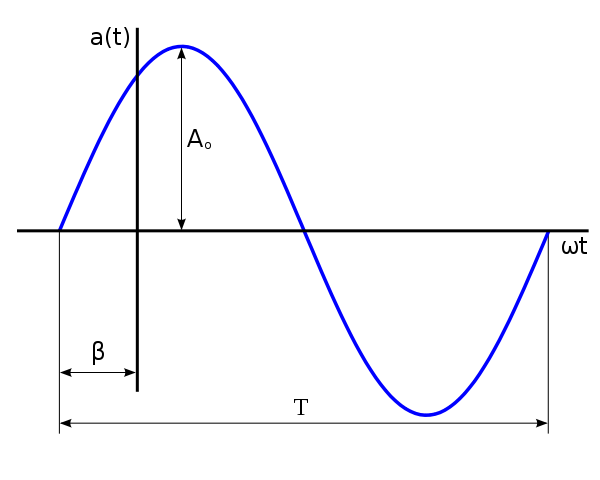
\includegraphics[scale=0.5]{Imagenes/600px-OndaSenoidal.png}
    \caption{Parámetros característicos de una oscilación sinusoidal.}
    \label{fig:ondaSenoidal}
\end{figure}



\begin{itemize}
    \item Cobre $1.72 x 10-8 [\Omega m]$ \citep{RS}
    \item Germanio puro  $0.60 [\Omega m]$ \citep{RS}
\item Silicio puro $2300 [\Omega m]$ \citep{RS}
\item  Grafeno $1 x 10-4 [\Omega m]$ \citep{Graf}
\end{itemize}

\subsubsubsection{Valores significativos}


A continuación se indican otros valores significativos de una señal sinusoidal:

\begin{itemize}

    \item Valor instantáneo (a(t)): Es el que toma la ordenada en un instante, t, determinado.

    
    \item Valor pico a pico (App): Diferencia entre su pico o máximo positivo y su pico negativo. Dado que el valor máximo de sen(x) es +1 y el valor mínimo es -1, una señal sinusoidal que oscila entre +A0 y -A0. El valor de pico a pico, escrito como AP-P, es por lo tanto (+A0)-(-A0) = 2×A0.

    \item Valor medio (Amed): Valor del área que forma con el eje de abscisas partido por su período. El valor medio se puede interpretar como el componente de continua de la oscilación sinusoidal. El área se considera positiva si está por encima del eje de abscisas y negativa si está por debajo. Como en una señal sinusoidal el semiciclo positivo es idéntico al negativo, su valor medio es nulo. Por eso el valor medio de una Oscilación sinusoidal se refiere a un semiciclo. Mediante el cálculo integral se puede demostrar que su expresión es la siguiente;

     \item  A_{med} = 2 A 0 π {\displaystyle A_{med}={2A_{0} \over {\pi }}} A_{{med}}={2A_{0} \over {\pi }}

    \item  Pico o cresta: Valor máximo, de signo positivo (+), que toma la oscilación sinusoidal del espectro electromagnético, cada medio ciclo, a partir del punto “0”. Ese valor aumenta o disminuye a medida que la amplitud “A” de la propia oscilación crece o decrece positivamente por encima del valor "0".

    \item Valor eficaz (A): El valor eficaz se define como el valor de una corriente (o tensión) continua que produce los mismos efectos calóricos que su equivalente de alterna. Es decir que para determinada corriente alterna, su valor eficaz (Ief) será la corriente continua que produzca la misma disipación de potencia (P) en una resistencia(R). Matemáticamente, el valor eficaz de una magnitud variable con el tiempo, se define como la raíz cuadrada de la media de los cuadrados de los valores instantáneos alcanzados durante un período:

        \item A = 1 T ∫ 0 T a 2 ( t ) d t {\displaystyle A={\sqrt {{1 \over {T}}{\int _{0}^{T}a^{2}(t)dt}}}} A={\sqrt {{1 \over {T}}{\int _{{0}}^{{T}}a^{2}(t)dt}}}
\end{itemize}

    Valor instantáneo (a(t)): Es el que toma la ordenada en un instante, t, determinado.

    Valor pico a pico (App): Diferencia entre su pico o máximo positivo y su pico negativo. Dado que el valor máximo de sen(x) es +1 y el valor mínimo es -1, una señal sinusoidal que oscila entre +A0 y -A0. El valor de pico a pico, escrito como AP-P, es por lo tanto (+A0)-(-A0) = 2×A0.

    Valor medio (Amed): Valor del área que forma con el eje de abscisas partido por su período. El valor medio se puede interpretar como el componente de continua de la oscilación sinusoidal. El área se considera positiva si está por encima del eje de abscisas y negativa si está por debajo. Como en una señal sinusoidal el semiciclo positivo es idéntico al negativo, su valor medio es nulo. Por eso el valor medio de una Oscilación sinusoidal se refiere a un semiciclo. Mediante el cálculo integral se puede demostrar que su expresión es la siguiente;


\begin{equation}
     A_{med} = 2 A 0 π {\displaystyle A_{med}={2A_{0} \over {\pi }}} A_{{med}}={2A_{0} \over {\pi }}

\end{equation}
   
    Pico o cresta: Valor máximo, de signo positivo (+), que toma la oscilación sinusoidal del espectro electromagnético, cada medio ciclo, a partir del punto “0”. Ese valor aumenta o disminuye a medida que la amplitud “A” de la propia oscilación crece o decrece positivamente por encima del valor "0".

    Valor eficaz (A): El valor eficaz se define como el valor de una corriente (o tensión) continua que produce los mismos efectos calóricos que su equivalente de alterna. Es decir que para determinada corriente alterna, su valor eficaz (Ief) será la corriente continua que produzca la misma disipación de potencia (P) en una resistencia(R). Matemáticamente, el valor eficaz de una magnitud variable con el tiempo, se define como la raíz cuadrada de la media de los cuadrados de los valores instantáneos alcanzados durante un período:


\begin{equation}
    A = 1 T ∫ 0 T a 2 ( t ) d t {\displaystyle A={\sqrt {{1 \over {T}}{\int _{0}^{T}a^{2}(t)dt}}}} A={\sqrt {{1 \over {T}}{\int _{{0}}^{{T}}a^{2}(t)dt}}}

\end{equation}
        
En la literatura inglesa este valor se conoce como R.M.S. (root mean square, valor cuadrático medio), y de hecho en matemáticas a veces es llamado valor cuadrático medio de una función. En el campo industrial, el valor eficaz es de gran importancia, ya que casi todas las operaciones con magnitudes energéticas se hacen con dicho valor. De ahí que por rapidez y claridad se represente con la letra mayúscula de la magnitud que se trate (I, V, P, etc.). Matemáticamente se demuestra que para una corriente alterna sinusoidal el valor eficaz viene dado por la expresión:

\begin{equation}
       A = A 0 2 {\displaystyle A={A_{0} \over {\sqrt {2}}}} A={A_{0} \over {{\sqrt 2}}}
\end{equation}

El valor A, tensión o intensidad, es útil para calcular la potencia consumida por una carga. Así, si una tensión de alterna, desarrolla una cierta potencia P en una carga resistiva dada, una tensión de continua de Vrms desarrollará la misma potencia P en la misma carga, por lo tanto Vrms x I = VCA x I (véase Potencia en corriente alterna).


%\subsection{Energía Eléctrica}

%Se denomina energía eléctrica a la forma de energía que resulta de la existencia de una diferencia de potencial entre dos puntos, lo que permite establecer una corriente eléctrica entre ambos cuando se los pone en contacto por medio de un conductor eléctrico. La energía eléctrica puede transformarse en muchas otras formas de energía, tales como la energía lumínica o luz, la energía mecánica y la energía térmica.\citep{EE}

%\subsection{Electricidad}

%La electricidad (del griego ήλεκτρον élektron, cuyo significado es ‘ámbar’) es el conjunto de fenómenos físicos relacionados con la presencia y flujo de cargas eléctricas. Se manifiesta en una gran variedad de fenómenos como los rayos, la electricidad estática, la inducción electromagnética o el flujo de corriente eléctrica. Es una forma de energía tan versátil que tiene un sinnúmero de aplicaciones, por ejemplo: transporte, climatización, iluminación y computación.\citep{Elec}

%La electricidad se manifiesta mediante varios fenómenos y propiedades físicas:\citep{Elec}


%\begin{itemize}
   

 %    \item Carga eléctrica: una propiedad de algunas partículas subatómicas, que determina su interacción electromagnética. La materia eléctricamente cargada produce y es influida por los campos electromagnéticos.\citep{Elec}
     
  %   \item Corriente eléctrica: un flujo o desplazamiento de partículas cargadas eléctricamente por un material conductor. Se mide en amperios.\citep{Elec}
     
   %  \item Campo eléctrico: un tipo de campo electromagnético producido por una carga eléctrica, incluso cuando no se está moviendo. El campo eléctrico produce una fuerza en toda otra carga, menor cuanto mayor sea la distancia que separa las dos cargas. Además, las cargas en movimiento producen campos magnéticos.\citep{Elec}
     
    % \item Potencial eléctrico: es la capacidad que tiene un campo eléctrico de realizar trabajo. Se mide en voltios.
    %Magnetismo: la corriente eléctrica produce campos magnéticos, y los campos magnéticos variables en el tiempo generan corriente eléctrica.\citep{Elec}

%\end{itemize}

\subsection{Error relativo y absoluto}

Existen dos maneras de cuantificar el error de la medida:\citep{ErrorEx}

\begin{itemize}
    \item  Mediante el llamado error absoluto, que corresponde a la diferencia entre el valor medido $fm$ y el valor real $fr$.
    \item Mediante el llamado error relativo, que corresponde al cociente entre el error absoluto y el valor real $fr$.\citep{ErrorEx}
\end{itemize}

   

Matemáticamente tenemos las siguientes expresiones:\citep{ErrorEx}\\


\begin{eqnarray}
    e_{abs}= f_m − f_r\\
    e_{rel}= \frac{f_m − f_r}{f_r} 
\end{eqnarray}
    \citep{ErrorEx}

Es importante notar que en las anteriores expresiones el valor real fr es una cantidad desconocida, por lo que el valor exacto del error absoluto y relativo es igualmente desconocido. Afortunadamente, normalmente es posible establecer un límite superior para el error absoluto y el relativo, lo cual soluciona a efectos prácticos conocer la magnitud exacta del error cometido.\citep{ErrorEx}

\section{Señal Senoidal}

En el primer experimento que se muestra en la figura \ref{fig:seno4.9497.1khzprim} se utilizó una señal con las siguientes características:\\

\begin{itemize}
    \item Vpp=4.9497 [V]
    \item $V_{RMS}$=7 [V]
    \item frecuencia= 1[kHz]
    \item periodo 1 [kHz]
\end{itemize}


\begin{figure}[h!]
    \centering
    
   
\begin{tikzpicture}
\begin{axis}[
    axis lines = left,
    xlabel = {t[ms]},
    ylabel = {V[V]},
]

\addplot
[thick=0.1cm,
    domain=0:2, 
    samples=100, 
    color=red,
]
{4.9497*sin(deg((2*3.1459*x))};
\addlegendentry{$4.9497 V_{pp}$}
%Here the blue parabloa is defined
%\addplot [
 %   domain=-10:10, 
  %  samples=100, 
    %color=blue,
   % ]
    %{x^2 + 2*x + 1};
%\addlegendentry{$x^2 + 2x + 1$}
 
\end{axis}
\end{tikzpicture}

\caption{Señal senoidal 4.9497 Vpp}
    \label{fig:seno4.9497.1khzprim}
\end{figure}

\section{Onda Triangular}

En el generador de funciones se generó una onda tipo triangular con las siguientes características:\\

\begin{itemize}
    \item Vpp=20 [V]
    \item Periodo= 0.5[ms]
\end{itemize}

En ella se observó el cambio de ángulo en la mitad del periodo al bajar 70\% del valor de la simetría.

\section{Señal Cuadrada}

En el osciloscopio se ingresó a través del generador de funciones una señal cuadrada de 2 [kHz] y $V_{RMS}=10[V]$, conociendo que $V_{RMS=\frac{V}{\sqrt{3}}$ podemos realizar la gráfica.\\

Se hicieron varias mediciones variando el ciclo de trabajo a 50\%, 80\% y 20\%


%####TAU#######
\begin{figure}[h!]
    \centering
    
   
\begin{tikzpicture}
\begin{axis}[
    axis lines = left,
    xlabel = {t[ms]},
    ylabel = {V[V]},
]

\addplot [
thick=0.1cm,
    domain=-(0.25):0, 
    samples=100, 
    color=blue,
]
{ 17.32};
\addplot [
thick=0.1cm,
    domain=0:(0.25), 
    samples=100, 
    color=blue,
]
{0};
\addplot [
thick=0.1cm,
    domain=(0.25):(2*0.25), 
    samples=100, 
    color=blue,
]
{ 17.32};
\addplot [
thick=0.1cm,
    domain=(2*0.25):(3*0.25), 
    samples=100, 
    color=blue,
]
{0};
\addplot [
thick=0.1cm,
    domain=(3*0.25):(4*0.25), 
    samples=100, 
    color=blue,
]
{ 17.32};

\addlegendentry{Ciclo de trabajo}
%Here the blue parabloa is defined
%\addplot [
 %   domain=-10:10, 
  %  samples=100, 
    %color=blue,
   % ]
    %{x^2 + 2*x + 1};
%\addlegendentry{$x^2 + 2x + 1$}
 
\end{axis}
\end{tikzpicture}
\caption{Señal cuadrada a 50\% ($\tau=0.25[ms]$)}
    \label{fig:senialCuadrada50porc}
 
\end{figure}


%####TAU#######
\begin{figure}[h!]
    \centering
    
   
\begin{tikzpicture}
\begin{axis}[
    axis lines = left,
    xlabel = {t[ms]},
    ylabel = {V[V]},
]

\addplot [
thick=0.1cm,
    domain=-(0.4):0, 
    samples=100, 
    color=blue,
]
{ 17.32};
\addplot [
thick=0.1cm,
    domain=0:(0.1), 
    samples=100, 
    color=blue,
]
{0};
\addplot [
thick=0.1cm,
    domain=(0.1):(0.5), 
    samples=100, 
    color=blue,
]
{ 17.32};
\addplot [
thick=1,
    domain=(0.5):(0.6), 
    samples=100, 
    color=blue,
]
{0};
\addplot [
thick=0.1cm,
    domain=(0.6):(1), 
    samples=100, 
    color=blue,
]
{ 17.32};

\addlegendentry{Ciclo de trabajo}
%Here the blue parabloa is defined
%\addplot [
 %   domain=-10:10, 
  %  samples=100, 
    %color=blue,
   % ]
    %{x^2 + 2*x + 1};
%\addlegendentry{$x^2 + 2x + 1$}
 
\end{axis}
\end{tikzpicture}
\caption{Señal cuadrada a 80\% ($\tau=0.4[ms]$)}
    \label{fig:senialCuadrada80porc}
 
\end{figure}


%####TAU#######
\begin{figure}[h!]
    \centering
    
   
\begin{tikzpicture}
\begin{axis}[
    axis lines = left,
    xlabel = {t[ms]},
    ylabel = {V[V]},
]

\addplot [
thick=0.1cm,
    domain=-(0.1):0, 
    samples=100, 
    color=blue,
]
{ 17.32};
\addplot [
thick=0.1cm,
    domain=0:(0.4), 
    samples=100, 
    color=blue,
]
{0};
\addplot [
thick=0.1cm,
    domain=(0.4):(0.5), 
    samples=100, 
    color=blue,
]
{ 17.32};
\addplot [
thick=0.1cm,
    domain=(0.5):(0.9), 
    samples=100, 
    color=blue,
]
{0};
\addplot [
thick=0.1cm,
    domain=(0.9):(1), 
    samples=100, 
    color=blue,
]
{ 17.32};

\addlegendentry{Ciclo de trabajo}
%Here the blue parabloa is defined
%\addplot [
 %   domain=-10:10, 
  %  samples=100, 
    %color=blue,
   % ]
    %{x^2 + 2*x + 1};
%\addlegendentry{$x^2 + 2x + 1$}
 
\end{axis}
\end{tikzpicture}
\caption{Señal cuadrada a 20\% ($\tau=0.1[ms]$)}
    \label{fig:senialCuadrada20porc}
 
\end{figure}


\section{Offset DC}

Se introdujo a la señal de la figura \ref{figura:senialCuadrada50porc} un corrimiento de:\\

\begin{itemize}
    \item 3 [V]DC
    \item -4 [V]DC
    \item 6 [V]DC
    \item -2 [V]DC
\end{itemize}

y se observó que la señal se desplazaba verticalmente dependiendo de los valores ingresados, para valores negativos la señal se desplazaba hacia abajo y para valores positivos la señal se desplazaba hacia arriba.


\section{Conclusiones}

La práctica de señales fué un buen ejercicio ya que se utilizaron diferentes instrumentos en el laboratorio para generar y observar varios tipos de señales como la senoidal, la cuadrada etc, y además de que se modificaron varios parámetros como lo es el voltaje pico a pico, la frecuencia, y se observaron los cambios en el osciloscopio.

%.\\[100cm]
\bibliographystyle{plain}
\bibliography{Referencias.bib}

\end{document}
